\subsection{UAP Algorithmus} \label{chap:UAP}
Der hier beschriebene Algorithmus zur Generierung einer \acrlong{uap} basiert auf dem Ansatz von Moosavi-Dezfooli et al. \cite{moosavi-dezfooli_universal_2017}. Ziel ist es, eine Perturbation zu entwickeln, die auf neue Bilder übertragbar ist. Der Algorithmus durchläuft iterativ eine Auswahl von Trainingsbildern und bestimmt jeweils den kürzesten Weg zur Entscheidungsgrenze jedes Bildes. Die dabei erzeugten Perturbationen werden aufsummiert, um eine universelle Perturbation zu erzeugen. Abbildung \ref{fig:uap-paper-figure2} aus Moosavi-Dezfooli et al. \cite{moosavi-dezfooli_universal_2017} illustriert dieses Vorgehen.

\begin{figure}[H]
    \centering
    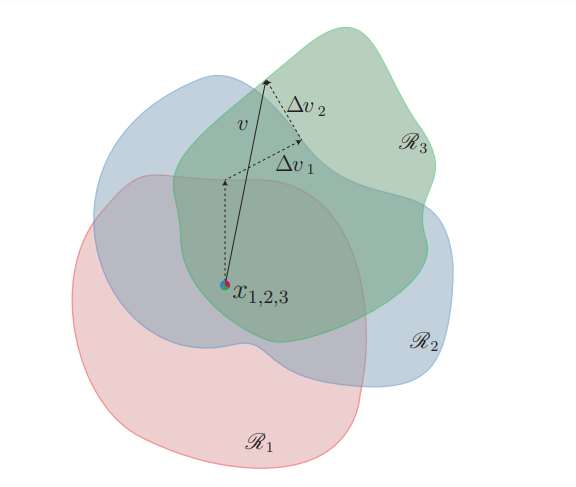
\includegraphics[width=0.6\linewidth]{01-images/04-methodik/UAP-figure2.png}
    \caption{Schematic representation of the proposed algorithm used to compute universal perturbations. In this illustration, data points $x1$, $x2$ and $x3$ are super-imposed, and the classification regions $R_{i}$ (i.e., regions of constant estimated label) are shown in different colors. Our algorithm proceeds by aggregating sequentially the minimal perturbations sending the current perturbed points $x_{i} + v$ outside of the corresponding classification region $R_{i}$ \cite{moosavi-dezfooli_universal_2017}}
    \label{fig:uap-paper-figure2}
\end{figure}

Bei der Generation der \acrshort{uap}s in dieser Thesis wird nur eine Teilmenge der positiv gelabelten Trainingsbilder verwendet. Zusätzlich wird durch die neu definierte Loss-Funktion nicht nur die neu generierte Änderung der Perturbation, sondern auch die totale Grösse der Perturbation bestraft. Die hier generierten \acrshort{uap}s sind im Gegensatz zum Paper von Moosavi-Dezfooli et al. \cite{moosavi-dezfooli_universal_2017} speziell darauf ausgelegt, bei einer binären Klassifikation positive Klassenbilder fälschlicherweise als negativ zu klassifizieren. 

\newpage
\subsubsection{Loss-Funktion \texorpdfstring{$L_{\text{UAP}}$}{Loss-Funktion L UAP}}
Das Optimierungsproblem von Moosavi-Dezfooli et al. \cite{moosavi-dezfooli_universal_2017} wird in dieser Implementierung durch eine selbst definierte Loss-Funktion gelöst, welche die $L_2$-Norm der Perturbation und die Inverse \acrlong{bce} Funktion minimiert. Durch die Minimierung der $L_2$-Norm der Perturbation wird sichergestellt, dass die erzeugte Perturbation minimal und somit weniger auffällig ist. Gleichzeitig sorgt die Minimierung der Inverse \acrlong{bce} dafür, dass die aktuelle Perturbation die Klassifikation des Bildes an die Entscheidungsgrenze bringt. Diese Kombination von Loss-Termen stellt sicher, dass die Perturbationen das attackierte Modell täuschen, aber so klein wie möglich sind.

Die Loss-Funktion optimiert $\Delta v_j$ und sieht wie folgt aus:
\begin{equation}
    L_{\text{UAP}} = \frac{1}{L_{\text{BCE,UAP}}(\hat{y}_i, \hat{y}_{i,\text{adv}}) + \epsilon} + \lambda_{norm} \cdot ||v_j + \Delta v_j||_2 
\label{eq:Loss L_UAP}
\end{equation}

Die verwendete \acrlong{bce} wird wie folgt definiert:
\begin{equation}
L_{\text{BCE,UAP}} = - (\hat{y}_i \cdot \log(\hat{y}_{i,\text{adv}}) + (1-\hat{y}_i) \cdot \log(1-\hat{y}_{i,\text{adv}}))
\label{eq:BCE_UAP}
\end{equation}

\begin{align*}
    \lambda_{norm}\text{:} &\text{ Regularisierungsparameter der Matrizennorm.} \\
    v_j\text{:} &\text{ \acrlong{uap}.} \\
    \Delta v_j\text{:} &\text{ Änderung der Perturbation } v_j \text{.} \\
    ||\cdot||_2\text{:} & \text{ $L_2$-Norm der Perturbation.} \\
    \hat{y}_i\text{:} &\text{ Vorhersage des Modells für das Originalbild, $f(x_{i})$.} \\
    \hat{y}_{i,\text{adv}}\text{:} &\text{ Vorhersage des Modells für das perturbierte Bild, $f(x_{i,\text{adv}})$.} \\
    \epsilon\text{:} &\text{ kleine positive Konstante für numerische Stabilität.}
\end{align*}

Für die Berechnung eines perturbierten Bildes $x_{i,\text{adv}}$ wird das Originalbild $x_i$ mit den Perturbationen $v_j$ und $\Delta v_j$ element-wise zusammenaddiert: 

\begin{equation}
    x_{i,\text{adv}} = x_i + v_j + \Delta v_j
    \label{eq:xadv}
\end{equation}

Der Algorithmus \ref{alg:uap-generierung} iteriert durch jedes Bild einzeln und sucht die Entscheidungsgrenze des aktuellen Bildes, was eine Batch-Grösse von 1 erfordert, wodurch kein Mittelwert in der Loss-Funktion berechnet wird.

Für $\epsilon$ wird ein kleiner Wert wie $10^{-6}$ gewählt, der eine Division durch 0 verhindert, wenn $L_{\text{BCE,UAP}}$ Null beträgt. Somit wird das Problem bei der Berechnung der ersten Perturbation gelöst, da zu diesem Zeitpunkt $v_j + \Delta v_j$ einen Nulltensor ergibt. 

\newpage

\subsubsection{Technische UAP Umsetzung} \label{chap:technische_umsetzung_uap}
Die technische Umsetzung des Prozesses zur Generierung der \acrshort{uap}s ist im folgenden Pseudocode beschrieben. Die Liste $v$ mit allen generierten Perturbationen wird zurückgegeben.

\begin{algorithm}[H]
\caption{Algorithmus für die Generierung von \acrlong{uap}}
\begin{algorithmic}[1]
\label{algo:UAP Algorithmus}
\STATE \textbf{initialize} Liste mit Perturbationen $v$
\FOR{Anzahl Perturbationen $j$}
    \STATE \textbf{initialize} Nulltensor $v_j$
    \WHILE{Fooling Rate $\text{FR}(k) < r$}
        \FOR{Bild $x_i$ $\in$ Trainingsdatensatz $X_{\text{train},+,1:n}$}
        \STATE \textbf{initialize} Nulltensor $\Delta v_j$
        \STATE \textbf{initialize} Integer $m_{\text{tries}} \gets 0$
            \WHILE{$(f(x_i)\geq k = f(x_{i,\text{adv}}) \geq k)$ \textbf{and} $m_{\text{tries}} < t$}         
            \STATE Aktualisiere $\Delta v_j$ mittels $L_{\text{UAP}}$: $$\Delta v_j \gets \Delta v_j - lr_{\text{UAP}} \cdot \frac{\partial L_{\text{UAP}}}{\partial \Delta v_j}$$
            \STATE Inkrementiere $m_{\text{tries}}$: $$m_{\text{tries}} \gets m_{\text{tries}} + 1$$
            \ENDWHILE
            \IF{$(f(x_i)\geq k \neq f(x_{i,\text{adv}}) \geq k)$}
                \STATE Addiere die Perturbation $\Delta v_j$ auf $v_j$: $$v_j \leftarrow v_j + \Delta v_j$$
            \ENDIF
        \ENDFOR
    \ENDWHILE
    \STATE Füge $v_j$ zur Liste $v$ hinzu:
    $$v \leftarrow v \cup {v_j}$$
\ENDFOR
\STATE \textbf{return} Liste mit Perturbationen $v$
\end{algorithmic}
\label{alg:uap-generierung}
\end{algorithm}

\begin{align*}
    j\text{:} &\text{ Anzahl zu generierende Perturbationsbilder.} \\
    n\text{:} &\text{ Anzahl Trainingsbilder.} \\
    t\text{:} &\text{ Anzahl Versuche, eine bildlokale Perturbation zu finden.}\\
    X_{\text{train},+,1:n}\text{:} &\text{ gemischte Teilmenge aller positiven gelabelten Trainingsbilder.} \\
    r\text{:} &\text{ gewünschte Mindesttäuschungsrate der Perturbation $v_j$ auf } X_{\text{train},+,1:n}.\\
    k\text{:} &\text{ Threshold der Entscheidungsgrenze. } k \in \left] 0; 1 \right[. \\
    p\text{:} &\text{ Normparameter der $L_2$-Norm, siehe \nameref{eq:BCE_UAP}.}\\
    \lambda_{norm},\epsilon\text{:} &\text{ siehe \nameref{eq:BCE_UAP}.}\\
    lr_{\text{UAP}}\text{:} &\text{ Lernrate der Gewichtsaktualisierung von $\Delta v_j$.}
\end{align*}

Ein Flow Chart zum \Gls{algorithmus} ist bei Abbildung \ref{fig:05-uap_algorithm} im Anhang zu finden. 

\subsubsection{Wahl des Regularisierungsparameters \texorpdfstring{$\lambda_{norm}$}{lambda\_norm}} \label{chap:wahl des Regularisierungsparameters}
Jedes Modell ist standardmässig unterschiedlich robust gegenüber \acrshort{uap}s. Deshalb kann nicht der gleiche Regularisierungsparameter $\lambda_{norm}$ für alle Modelle gewählt werden. Wird dieser Parameter zu hoch gewählt, wird die Generierung der \acrshort{uap}s instabil, sodass die gewünschte Schwelle der Entscheidungsgrenze $k$ nicht erreicht werden kann. Jedoch darf $\lambda_{norm}$ nicht zu klein gewählt werden, da ein kleinerer Wert zu einer geringen Bestrafung grosser Werte in den Perturbationen führt und dadurch die Perturbationen grösser werden. Aufgrund dieses Trade-offs wird ein Wert gesucht, welcher so gross wie möglich ist, jedoch noch eine stabile Generation der \acrshort{uap}s ermöglicht.

Der Ansatz zur Wahl des Parameters $\lambda_{norm}$ verläuft wie folgt: Die Untersuchung beginnt mit dem Wert 0.01, wobei das Verhalten des Algorithmus analysiert wird. Erweist sich dieser Wert als stabil, indem die Entscheidungsgrenze erreicht wird, erfolgt eine Erhöhung von $\lambda_{norm}$ auf 0.02 mit anschliessender Wiederholung des Verfahrens. Anschliessend werden die Werte 0.05, 0.1, 0.2, 0.5 und 1 systematisch getestet. Wenn ein Wert sich als instabil erweist, wird der vorherige Wert festgelegt. Wenn der Wert 1 sich als stabil erweist, wird er gewählt. Sollte sich der Ausgangswert 0.01 bereits als instabil erweisen, werden kleinere Abstufungen wie 0.005, 0.002, 0.001, 0.0005 usw. in Betracht gezogen.

In der Tabelle \ref{tab:Regularisierungsparameter} werden die gewählten Werte erfasst:

\begin{table}[H]
    \centering
    \begin{subtable}{0.45\linewidth}
        \centering
        \begin{tabular}{l|l}
            \hline
            \textbf{Modell} & \textbf{$\lambda_{norm}$} \\ 
            \hline
            ResNet18 & 1 \\
            \hline
            ResNet50 & 0.05 \\
            \hline
            DenseNet121 & 0.2\\
            \hline
            DenseNet169 & 0.2 \\
            \hline
            EfficientNetV2-S & 1\\
            \hline
            EfficientNetV2-M & 1\\
        \end{tabular}
        \caption{$\lambda_{norm}$ für den MRI Datensatz}
        \label{tab:BrainTumor}
    \end{subtable}%
    \hspace{0.05\linewidth} % Adjust horizontal space between tables
    \begin{subtable}{0.45\linewidth}
        \centering
        \begin{tabular}{l|l}
            \hline
            \textbf{Modell} & \textbf{$\lambda_{norm}$} \\ 
            \hline
            ResNet18 & 0.02 \\
            \hline
            ResNet50 & 0.05 \\
            \hline
            DenseNet121 & 0.02\\
            \hline
            DenseNet169 & 0.005 \\
            \hline
            EfficientNetV2-S & 0.02\\
            \hline
            EfficientNetV2-M & 0.0002\\
        \end{tabular}
        \caption{$\lambda_{norm}$ für den COVIDx CXR-4 Datensatz}
        \label{tab:COVIDxCXR4}
    \end{subtable}
    \caption{Gewählte  Regularisierungsparameter $\lambda_{norm}$}
    \label{tab:Regularisierungsparameter}
\end{table}

Hier lässt sich bereits beobachten, dass die gewählten Regularisierungsparameter für die Modelle des MRI-Datensatzes im Vergleich zum COVIDx CXR-4 Datensatz höher gewählt wurden. Daraus lässt sich schliessen, dass Modelle, die auf dem MRI Datensatz trainiert wurden, anfälliger auf kleine Perturbationen sind, während Modelle, die auf dem COVIDx CXR-4 Datensatz trainiert wurden, grössere Perturbationen benötigen, um das Abbruchkriterium zu erreichen.

\paragraph{Automatisierter Ansatz}
Alternativ könnte für die Wahl des Regularisierungsparameters $\lambda_{norm}$ ein automatisierter Ansatz verwendet werden, der die Werte granularer durchsucht. In dieser Thesis wurde gegen einen solchen Ansatz entschieden, da die Programmierung eines entsprechenden Algorithmus zeitintensiver wäre als die manuelle Ermittlung der Werte.
